% % % % % % % % % % % % % % % % % % % % % % % % % % % % % % % % % % % % % % % %
% LaTeX4EI Template for Cheat Sheets                                Version 1.1
%
% Authors: Markus Hofbauer
% Contact: info@latex4ei.de
% Encode: UTF-8
% % % % % % % % % % % % % % % % % % % % % % % % % % % % % % % % % % % % % % % %


% ======================================================================
% Document Settings
% ======================================================================

% possible options: color/nocolor, english/german, threecolumn
% defaults: color, english
\documentclass[english]{latex4ei/latex4ei_sheet}

% set document information
\title{Digitale Schaltungen}
\author{LaTeX4EI}                    % optional, delete if unchanged
\myemail{info@latex4ei.de}           % optional, delete if unchanged
\mywebsite{www.latex4ei.de}          % optional, delete if unchanged


% ======================================================================
% Begin
% ======================================================================
\begin{document}

\IfFileExists{git.id}{\input{git.id}}{}
\ifdefined\GitRevision\mydate{\GitNiceDate\ (git \GitRevision)}\fi

% Title
% ----------------------------------------------------------------------
\maketitle   % requires ./img/Logo.pdf


% Section
% ----------------------------------------------------------------------
\section{Transistorgleichungen}

\subsection{Bipolar}
$I_F = I_{ES}\left(\exp\left(\frac{U_{BE}}{U_T}\right)-1\right)$\\
Vorteil: bessere Treiberverstärkung durch Exponentialfunktion
Nachteile:\begin{itemize}
	\item hohe Verlustleistung
	\item langsames Abschalten durch Sättigung mit Ladungsträgern $\rightarrow$ ECL-Schaltung / Differentielles ECL / Feedback-ECL Differenzverstärker
\end{itemize}

\subsection{MOS-Transistoren}
 
Verstärkung: \framebox{
	$\beta = K' \frac{W}{L} \text{ mit } K' = \frac{\mu \varepsilon_{ox} \varepsilon_0}{t_{0x}} \qquad [\beta]=\frac{A}{V^2}$ 
} \\
\begin{tabular} {r | l}
	Kanalweite & W  \\
	Kanallänge & L  \\
	Elektronenbeweglichkeit & $\mu_n \approx 250 \cdot 10^{-4} \frac{m^2}{Vs}$\\
	 & $\mu_p \approx 100 \cdot 10^{-4} \frac{m^2}{Vs}$ \\
	rel. Dielektrizität des Gateoxyds & $\varepsilon_{ox} \approx 3,9$ \\
	Dielektrizitätskonstante & $\varepsilon_0 = 8.8541878 \cdot 10^{-12} \frac{\mathrm{A\,s}}{\mathrm{V\,m}}$ \\
	Gateoxyddicke & $t_{ox}$ \\
	Verstärkung & $\beta = \frac{\mu_n \varepsilon_{ox} \varepsilon_0}{t_{ox}} \cdot \frac{W}{L} = K' \frac{W}{L}$ \\
	Kapazität & $C_G = \varepsilon_{ox} \varepsilon_0 \frac{WL}{t_{ox}}$ \\
	Verzögerungszeit & $t_{pHL} \propto \frac{C_L t_{ox} L_p}{W_p \mu_p \varepsilon_{ox} (V_{DD} - |V_{th}|)}$ \\
\end{tabular}
\begin{itemize}
	\item große Kanalweite $\Ra$ große Drain-Störme \\ $\Ra$ schnelle Schaltgeschwindigkeit (da $i_d \propto \beta \propto \frac{W}{L}$) \\
	Aber: große Fläche.
	\item nMos schaltet schneller als pMOS, da nMOS und pMOS unterschiedliche Majoritätsladungsträger haben. Die Beweglichkeit der Löcher ist im Allgemeinen geringer als die der Elektronen. 
	\item nMOS zum Entladen, pMOS zum Aufladen
\end{itemize}

\textbf{nMos} (p-dotiertes Substrat, n-dotierte Drain/Source), schlechter pull up (Pegeldegenerierung)
\begin{equation*}
\!\!\! I_d = \begin{cases}
0, &\text{ für }  U_{gs} - U_{th} \le 0 \qquad \qquad  \text{(Sperrber.)}\\[0.2em]
\beta [(u_{gs} - U_{th}) \cdot u_{ds} - \frac{1}{2} u_{ds}^2] , &\text{ für }  0 \le U_{gs} - U_{th} \ge u_{ds} \  \text{(linearer Ber.)}\\\\[0.2em]
\frac{1}{2} \beta \cdot (u_{gs} - U_{th})^2, &\text{ für }  0 \le U_{gs} - U_{th} \le u_{ds} \  \text{(Sättigungsber.)}\\
\end{cases}
\end{equation*}
\textbf{pMos} (n-dotiertes Substrat, p-dotierte Drain/Source), schlechter pull down (Pegeldegenerierung)
\begin{equation*}
\!\!\! I_d = \begin{cases}
0, &\text{ für }  U_{gs} - U_{th} \ge 0\\[0.2em]
- \beta [(u_{gs} - U_{th}) \cdot u_{ds} - \frac{1}{2} u_{ds}^2] , &\text{ für }  0 \ge U_{gs} - U_{th} \le u_{ds}\\\\[0.2em]
- \frac{1}{2} \beta \cdot (u_{gs} - U_{th})^2, &\text{ für }  0 \ge U_{gs} - U_{th} \ge u_{ds}\\

\end{cases}
\end{equation*}

\section{Sequentielle Logik}

\begin{tabular}{c|l}
	$t_{\text{Setup}}$ & Stabilitätszeit vor der aktiven Taktflanke\\
	$t_{\text{hold}}$ & Stabilitätszeit nach  der aktiven Taktflanke\\
	$t_{\text{c2q}}$ & Eingang wird spätestens nach $t_{c2q}$ am Ausgang verfügbar\\
	Min. Taktperiode &  $t_{clk} \ge t_{1,c2q} + t_{logic,max} + t_{2,setup}$ \\
	 & (bei Verletzung: Pipelinestufe einfügen, aber dadurch höhere Latenz) \\
	Max. Taktfrequenz & $f_{max} = \left\lfloor \frac{1}{t_{clk}} \right\rfloor$ \qquad (Nicht aufrunden) \\
	Holdzeitbedingung & $t_{hold} \le t_{c2q} + t_{logic,min}$  $\ra$ (bei Verletzung zwei Inverter einfügen)\\
	Durchsatz & $\frac{1 \text{Sample}}{t_{clk,pipe}} = f$ \\
	Latenz & $t_{clk} \cdot \#$Pipelinestufen (das zwischen den FFs) \\
\end{tabular}

\subsection{Zeitmessungen}

Ersatzwiderstand für den Transistor: $R_{\text{on}} \approx \frac{1}{\beta (\abs{U_{\text{gs,p}}}-\abs{U_{\text{th,p}}})}$

Guardband: $t_{\text{guard}} = t_{\text{clk}}-t_{\text{p,max}}$

\subsubsection{Propagation-Delay}
Zeit, die beim Umschalten zwischen 50\% der Eingangsspannung und 50\% der Ausgangsspannung vergeht

$t_p = \frac{t_{\text{p,LH}} + t_{\text{p,HL}}}{2} = \ln{2}R_{\text{on}}C_L$\\
Für eine Treiberstufe: $t_p = \ln{2}\frac{R_{\text{on}}}{S}(S\cdot C_{\text{int}} + C_L)$ mit Kanalweitenskalierung $S=\sqrt[N]{\frac{C_L}{C_g}}$\\ \\

$t_{\text{p,LH}} \approx \frac{C_L t_{\text{ox}}L}{W\mu\varepsilon(U_{\text{DD}}-\abs{U_{\text{th,p}}})}$
Falls $W\rightarrow\infty$ gilt trotzdem $t\neq 0$, da interne Gate-Kapazität so wächst!

\subsubsection{Rise- and Fall-Time}
Zeit, die beim Umschalten eines Signals von 10\% auf 90\% vergeht

\subsubsection{Lastkapazitäten}
Umladen von parasitären Lastkapazitäten braucht Zeit.
Diese setzen sich wie folgt zusammen:
\begin{itemize}
	\item Eingangs/Gate-Kapazität der nachfolgenden Stufe
	\item Drain-Kapazität
	\item Leiterbahn-Kapazitäten
\end{itemize}

\subsubsection{Elmore-Delay}
Es müssen alle Kapazitäten berücksichtigt werden und alle Widerstände auf gemeinsamen Pfaden. Hier sollen dann die RC Konstanten aufaddiert werden.\\
Beispiel: $\tau = R_C\cdot C_2 + (R_C+R_B)C_1+(R_C+R_B+R_A)C_L$
%TODO Bild aus VL einfügen

\subsection{Pipelining} % (fold)
Nur bei synchronen(taktgesteuerten) Schaltungen möglich!
\begin{itemize} \itemsep0pt
	\item Aufteilen langer kombinatorischer Pfade durch Einfügen zusätzlicher Registerstufen\\
	$\ra$ Möglichst Halbierung des längsten Pfades
	\item Zeitverhalten beachten (evtl. Dummy-Gatter einfügen)
	\item Durchsatz erhöht sich entsprechend der Steigerung der Taktfrequenz
	\item Gesamtlatenz wird eher größer
	\item Taktfrequenz erhöht sich
\end{itemize}

\subsection{Latch}
%TODO Schaltbild einfügen

SB = RB = Q = QB $\Rightarrow$ Latch schwingt \\
$t_{\text{rise}} \neq t_{\text{fall}} \Rightarrow$ Schwingung klingt ab

\section{Statische CMOS-Schaltungen}
XXX

\section{Pass-Transistor-Logik}

\begin{tablebox}{l|l}
	Vorteile & Nachteile\\
	\brule
	Wenige Transistoren & zusätzliche Inverter\\
	& oder Transmission Gates für Pegelregeneration\\
	Kleiner Flächenverbrauch & Verdrahtungsaufwand hoch\\
	Geringe Verlustleistung & Langsam
\end{tablebox}

\subsection{Erweitertes KV-Diagramm}

Einträge (0 oder 1) des KV-Diagramms werden durch die jeweilige DNF für den Einseintrag ergänzt. Hierdurch können anschließend einfach die Einträge mit den gleichen DNFs gefunden werden.

%TODO Bild einfügen

\section{Dynamische CMOS-Schaltungen}

\begin{tablebox}{l|l}
	Vorteile & Nachteile\\
	\brule
	Nur ein Logikblock & Ladungsverlust durch Leckströme und\\
	statt zwei benötigt & und Charge-Sharing\\
	
\end{tablebox}

Damit die Pegelregeneration gewährleistet ist, sollten Gatter immer abwechselnd mit NMOS und PMOS-Technik kaskadiert werden. Alternativ kann auch ein statische Schaltung benutzt werden.

%TODO Beispielbild

\subsection{Master-Slave-Flip-Flop}

%TODO Bild einfügen

Achtung mit Clock-Gating bei dynamischen Registern, sonst Datenverlust durch Leckströme

\section{CMOS Verlustleistung}
Inverterschaltvorgang $V_A: 0 \ra 1$:\\
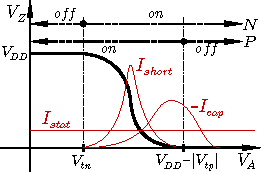
\includegraphics{img/ds/char_inverter.pdf}

\subsection{Dynamische Verlustleistung}
 \qquad \ $P_{dyn} = P_{cap} + P_{short}$\\
\begin{tabular}{ll}
	\quad Kapazitive Verluste \qquad \ \quad \ & $P_{cap} = \alpha_{01} f C_L V_{DD}^2$\\
	\quad Kurzschlussstrom	& $P_{short} = \alpha_{01} f \beta_n \tau (V_{DD} - 2V_{tn})^3$\\[0.8em]
	\quad Schalthäufigkeit & $\alpha_{0 \rightarrow 1} = \frac{\text{Schaltvorgänge(pos. Flanke)}}{\text{\# Betrachtete Takte}}$\\
	\quad Schalthäufigkeit (periodisch) & $\alpha = \frac{f_\text{switch}}{f_\text{clk}}$\\
\end{tabular}\\
Abhängig von den Signalflanken, mit Schaltfunktionen verknüpft\\ 
$\approx \;$ $V_{DD} 1/\propto $ Schaltzeit: $\frac{V_{DD2}}{V_{DD1}} = \frac{t_{D1}}{t_{D2}}$ (bei Schaltnetzen $t_{log}$)\\
\textbf{Verzögerungszeit} $\propto$ $\frac{C_Lt_{ox}L_p}{W_p\mu_p\varepsilon(V_{DD} - V_{th})}$

Steigend mit: Kapazitiver Last, Oxiddicke, Kanallänge, Schwellspannung

Sinkend mit: Kanalweite, Ladungsträger Beweglichkeit, Oxyd Dielektrizität, Versorgungsspannung \\ \\
\subsection{Statische Verlustleistung}
Abhängigkeit: $V_{DD}\uparrow:P_{stat}\uparrow$ \qquad $V_{th}\uparrow:P_{stat}\downarrow$ \quad (aber nicht proportional)\\
Sub-Schwellströme:\\
$I_D= I_0 \exp\left(\frac{V_{\text{gs}}-V_T}{nV_{\text{Temp}}}\right) \left(1-\exp\left(V_{\text{ds}}-V_{\text{Temp}}\right)\right)$ für $V_{\text{gs}} < V_{\text{T}}$\\
Leckströme/Gate-Ströme (Sperrströme, da Gate-Oxit nicht richtig isoliert):\\
$I_{\text{Gate}} \sim \exp\left(t_{\text{ox}}^{-1}\right)$\\
\\
Optimierung durch:
\begin{itemize}
	\item Clock-Gating: Nicht benötigte Blöcke können innerhalb einer Taktflanke an- und abgeschaltet werden
	\item Power-Gating: Nicht benötigte Bereiche können abgeschaltet werden, Daten müssen jedoch zuvor abgespeichert werden
	\item Dynamic Voltage Frequency Scaling: Versorgungsspannung und Frequenz $\downarrow \Rightarrow$ Dynamic Power $\downarrow$
\end{itemize}

Die Schwellspannung kann durch Substratvorspannung (Bulk) verändert werden
%TODO verschieben? und eventuell Bild

\section{Speicher}
\subsection{DRAM-Zelle}
%TODO Bild
Information wird nur temporär in Kondensator gespeichert. Es muss regelmäßig aufgefrischt werden.
\subsection{SRAM-Zelle}
%TODO
TODO
\subsection{Flash-Zelle}
%TODO Bild
Elektronen werden durch eine hohe Spannung am Gate und Drain auf das Floating-Gate gezogen. Zur Speicherung wird keine Spannung benötigt. Beim Lesen mit mittlerer Spannung verschieben die Elektronen im Floating-Gate die Thresholdspannung.\\
Das Oxid wird beim Laden/Entladen beschädigt (geringe Lebenszeit), deswegen muss die Nutzung auf allen Speicherzellen verteilt werden.
\subsection{Phase-Change-Memory}
Bei Raumtemperatur kann das Phase-Change-Material sich bei Raumtemperatur stabil in zwei Zuständen befinden: Amorph und Kristallin. Die Zustände können durch eine Reset(Melt)temperatur bzw. der Crystaltemperatur gewechselt werden. 

%TODO Bild

\section{Fehlertoleranz}
Es können verschiedene Fehler entstehen:
\begin{itemize}
	\item Manufacturing Variability ($V_T$)
	\item Soft-Errors (Fehler, die auftreten und wieder verschwinden)
	\item Alterung und Transistorperformanz (langsamer werdend)
\end{itemize}

Fehlermodelle:\\
\textbf{a) Permanente Fehler:} Stuck-At(0/1), Stuck-Open, Bridge-Fault (Ursache: Elektromigration)\\
\textbf{b) Transiente Fehler:} Kurzfristig falsche Werte, Single Event Transient/Upset (Ursache: natürliche Strahlung bsplw. alpha-Strahlen)\\
Single Event Transient: kurzer falscher Spannungswert durch Zeitverletzung durch Nebensprechen oder Alterung\\
Single Event Upset: Übernahme eines falschen Wertes durch Umkippen in ein FlipFlop

\subsection{Fehlermaskierung}

\textbf{Fehlersensitivität:} Fehler ist am Ausgang bemerkbar\\
\textbf{Logikmaskierung:} Wert ist irrelevant für den Ausgang\\
\textbf{Transiente Maskierung:} Logische Maskierung an späterer Stufe verhindert falsche Ausbreitung\\

\section{Synchrone und Ansynchrone Schaltungen}




% ======================================================================
% End
% ======================================================================
\end{document}
